\documentclass[letterpaper,final,12pt,reqno]{amsart}

\usepackage[total={6.3in,9.2in},top=1.1in,left=1.1in]{geometry}

\usepackage{bm}
\usepackage{empheq}
\usepackage[dvipsnames]{xcolor}
\usepackage{graphicx}
\usepackage{verbatim,fancyvrb}
\usepackage{tikz}

% hyperref should be the last package we load
\usepackage[pdftex,
colorlinks=true,
plainpages=false, % only if colorlinks=true
linkcolor=blue,   % only if colorlinks=true
citecolor=Red,   % only if colorlinks=true
urlcolor=black     % only if colorlinks=true
]{hyperref}

\renewcommand{\baselinestretch}{1.05}

\newcommand{\ddt}[1]{\ensuremath{\frac{\partial #1}{\partial t}}}
\newcommand{\ddx}[1]{\ensuremath{\frac{\partial #1}{\partial x}}}
\newcommand{\ddy}[1]{\ensuremath{\frac{\partial #1}{\partial y}}}
\newcommand{\pp}[2]{\ensuremath{\frac{\partial #1}{\partial #2}}}
\renewcommand{\t}[1]{\texttt{#1}}
\newcommand{\Matlab}{\textsc{Matlab}\xspace}
\newcommand{\eps}{\epsilon}
\newcommand{\RR}{\mathbb{R}}

\newcommand{\grad}{\nabla}
\newcommand{\Div}{\nabla\cdot}
\newcommand{\trace}{\operatorname{tr}}


\newcommand{\hbn}{\hat{\mathbf{n}}}

\newcommand{\bg}{\mathbf{g}}
\newcommand{\bn}{\mathbf{n}}
\newcommand{\bu}{\mathbf{u}}
\newcommand{\bv}{\mathbf{v}}
\newcommand{\bx}{\mathbf{x}}

\newcommand{\bX}{\mathbf{X}}



\begin{document}
\graphicspath{{figures/}}

\title[Appendix A]{Appendix A: A finite element Stokes solver \\ for glacier flow}

\author{Ed Bueler}

\maketitle

\vspace{-8mm}
\begin{center}
\footnotesize
\emph{version: \today~for McCarthy 2022}
\end{center}

\thispagestyle{empty}
\bigskip

\renewcommand{\thefigure}{A\arabic{figure}}
\renewcommand{\theequation}{A\arabic{equation}}
\renewcommand{\thesection}{A.\arabic{section}}

This is an appendix to my notes \emph{Numerical modelling of glaciers, ice sheets, and ice shelves}---here called ``the notes''---for the International Summer School in Glaciology in McCarthy, Alaska.

First we state the Stokes model for ice flow, with glacier-suitable boundary conditions, for example as in Figure \ref{fig:glacier}, including the slab-on-a-slope case.  (The slab exact solution is useful both for verification purposes and as a source of boundary conditions for general cases.)  We then derive the \emph{weak form} of the Stokes problem.  A brief overview of \emph{finite element} (FE) methods, based on such weak forms, follows.  Our particular FE method uses an unstructured mesh of triangular elements, on any planar region, to solve the Glen-Stokes problem by a stable \emph{mixed element} method with distinct approximating spaces for velocity and pressure.  We demonstrate a numerical solution for the instantaneous velocity and pressure.  Then we describe a moving-mesh scheme to solve the surface kinematical equation, and demonstrate an evolving glacier shape.

\begin{figure}[h]
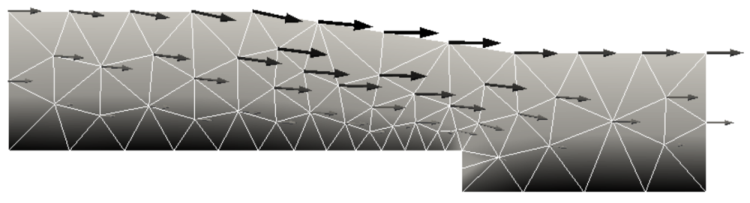
\includegraphics[width=\textwidth,angle=-5.7296]{stepflowlin}  % 0.1 radian = 5.7296 degrees
\caption{A 2D glacier flowing over a bedrock step.  Arrows show velocity $\bu$ and shading is by pressure $p$.}
\label{fig:glacier}
\end{figure}

Our numerical model is in short Python codes, documented at the end, which exploit four advanced open source tools and libraries:
\begin{itemize}
\item Firedrake, an FE library \hfill \url{https://www.firedrakeproject.org/}
    \begin{itemize}
    \item[$\circ$] inside Firedrake is PETSc, a solver library \hfill \url{https://petsc.org/}
    \end{itemize}
\item Gmsh, a mesh generator \hfill \url{http://gmsh.info/}
\item Paraview, a visualization tool \hfill \url{https://www.paraview.org/}
\end{itemize}


\section{Glen-Stokes model} \label{sec:stokes}

Recall the Glen-Stokes model in equations (3)--(5) from the notes.  This model, also described in \cite{GreveBlatter2009,JouvetRappaz2011}, applies on a 2D or 3D domain $\Omega$ which must have a piecewise smooth boundary (so that we may apply boundary conditions).  Allowing any Glen exponent $n\ge 1$, the equations are:
\begin{align}
- \nabla \cdot \tau + \nabla p &= \rho \bg &&\text{\emph{stress balance}} \label{forcebalance} \\
\nabla \cdot \bu &= 0 &&\text{\emph{incompressibility}} \label{incompressible} \\
D\bu &= A_n |\tau|^{n-1} \tau &&\text{\emph{Glen flow law}} \label{flowlaw}
\end{align}
The notation here generally follows Table 1 in the notes, including velocity $\bu$, pressure $p$, ice density $\rho$, acceleration of gravity $\bg$, deviatoric stress tensor $\tau$ and strain rate tensor $D\bu$.  Tensors $D\bu$ and $\tau$ are symmetric and have trace zero.  Recall that $D\bu$ is the symmetric part of the tensor velocity derivative $\grad \bu$:
\begin{equation}
(D\bu)_{ij} = \frac{1}{2} \left(\grad\bu + \grad\bu^\top\right) = \frac{1}{2} \left((u_i)_{x_j} + (u_j)_{x_i}\right) \label{strainrate}
\end{equation}
The full (Cauchy) stress tensor $\sigma$ is the deviatoric stress tensor $\tau$ minus the pressure,
\begin{equation}
    \sigma = \tau - p\,I,  \label{cauchystress}
\end{equation}
so equation \eqref{forcebalance} simply says $-\Div \sigma = \rho \bg$.  One may derive from \eqref{cauchystress} that $p = -\frac{1}{3} \trace(\sigma)$ (in 3D), thus the pressure is the negative of the average normal stress.  By definition $\Div\tau$ in \eqref{forcebalance} is a vector with components which are the divergences of the rows:
\begin{equation}
    \left(\nabla \cdot \tau\right)_i = \left(\tau_{i1}\right)_{x_1} + \left(\tau_{i2}\right)_{x_2} + \left(\tau_{i3}\right)_{x_3}  \label{divtaudefn}
\end{equation}
Note $\nabla\cdot \tau$, $\nabla p$, and $\bg$ are regarded as column vectors.

The viscosity form of \eqref{flowlaw} can also be found in the notes:
\begin{equation}
\tau = 2\nu D\bu = B_n |D\bu|^{\frac{1}{n} - 1} D\bu  \label{viscflowlaw}
\end{equation}
Here $B_n = (A_n)^{-1/n}$ is the $n$-dependent ice hardness in units $\text{Pa}\,\text{s}^{1/n}$.  The tensor norm notation used in \eqref{flowlaw}  and \eqref{viscflowlaw} is defined as follows, with the summation convention:
\begin{align*}
|\tau|^2 = \frac{1}{2} \trace\left(\tau^2\right) = \frac{1}{2} \tau_{ij} \tau_{ij}, \qquad |D\bu|^2 = \frac{1}{2} \trace\left((D\bu)^2\right) = \frac{1}{2} (D\bu)_{ij} (D\bu)_{ij}
\end{align*}

Using \eqref{viscflowlaw} we can eliminate $\tau$ from equation \eqref{forcebalance}, thereby rewriting the system in terms of velocity $\bu$ and pressure $p$ only:
\begin{align}
- \nabla \cdot \left(B_n |D\bu|^{\frac{1}{n} - 1} D\bu\right) + \nabla p &= \rho \mathbf{g} \label{stokes} \\
\Div \bu &= 0 \label{incompagain}
\end{align}
This system is the preferred Glen-Stokes model.  A solution is a pair $(\bu,p)$.

From now on we suppose the domain $\Omega$ is 2D, so points are denoted $(x,z)$.  (Relative to 3D: $y=0$, $\partial/\partial y=0$, $v=0$, and $\bu=\left<u,w\right>$.)  Also we will assume the force of gravity is at an angle $\alpha$ with the $z$-direction so $\bg = \left<g\sin\alpha,-g\cos\alpha\right>$ where $g=|\bg|$.

Certain glacier-suitable velocity and stress boundary conditions will be used here.  We assume that the base, top, inflow, and outflow boundaries can all be identified.  On the base we require no slip:
\begin{align}
\bu &= 0  &&\text{\emph{base}} \label{basebc} \\
\intertext{On the top we set a condition of zero applied stress, i.e.~$\sigma\hbn=0$:}
\left(B_n |D\bu|^{\frac{1}{n} - 1} D\bu - pI\right) \hbn &= 0  &&\text{\emph{top}} \label{topbc} \\
\intertext{The left-side inflow boundary has outward normal $\hbn=\left<-1,0\right>$ in our case, and on this surface we set a nonzero inflow velocity:}
\bu &= \left<f(z),0\right>  &&\text{\emph{inflow}} \label{inflowbc} \\
\intertext{(The function $f(z)$ will satisfy the slab-on-slope equations for a specific thickness $H_{\text{in}}$ at the inflow; see below.)  On an outflow boundary, where $\hbn=\left<1,0\right>$, we set a nonzero hydrostatic normal stress using the (varying) ice thickness $H_{\text{out}}$ at the outflow:}
\left(B_n |D\bu|^{\frac{1}{n} - 1} D\bu - pI\right) \hbn &= C_{\text{out}} \big<- \rho g \cos\alpha (H_{\text{out}}-z),  \notag && \\
    &\qquad\qquad \rho g\sin\alpha (H_{\text{out}}-z)\big> && \text{\emph{outflow}} \label{outflowbc}
\end{align}
The constant $C_{\text{out}} $ is adjusted so that the total applied stress is equal to its value for the input ice thickness $H_{\text{in}}$, thus $C_{\text{out}} = (H_{\text{in}}/H_{\text{out}})^2$.


\section{Slab-on-slope solutions}  \label{sec:slab}

Testing a numerical model requires verification tools, namely exact solutions, so here we recapitulate the slab-on-slope construction given in the notes.  This time we allow any Glen exponent $n$.  We will construct inflow and outflow boundary conditions, for use when solving for more general flows, from this case.

Using component notation for 2D, equations \eqref{stokes}, \eqref{incompagain} become the following Glen-Stokes model in coordinates $(x,z)$ and velocity components $\bu=\left<u,w\right>$:
\begin{align}
- \left(B_n |D\bu|^{\frac{1}{n}-1} u_x\right)_x - \left(\frac{1}{2} B_n |D\bu|^{\frac{1}{n}-1} \left(u_z+w_x\right)\right)_z + p_x &= \rho g\sin\alpha \label{planestressx} \\
- \left(\frac{1}{2} B_n |D\bu|^{\frac{1}{n}-1} \left(u_z+w_x\right)\right)_x - \left(B_n |D\bu|^{\frac{1}{n}-1} w_z\right)_z + p_z &= -\rho g\cos\alpha \label{planestressz} \\
u_x + w_z &= 0 \label{planeincomp}
\end{align}
The strain-rate norm expands to
\begin{equation}
    |D\bu|^2 = \frac{1}{2} \left(u_x^2 + \frac{1}{2}(u_z+w_x)^2 + w_z^2\right)  \label{planeDnorm}
\end{equation}

Consider a slab with fixed ($x$-independent) values of the bed elevation $b$ and the surface elevation $h$, so the domain is $\Omega = \{(x,z)\,|\,b < z < h\}$.  (This describes either an infinitely-long or a periodic slab flow.)  Assume that the boundary stresses are also $x$-independent.  Then there is no variation in $x$, i.e.~$\partial/\partial x=0$, so the system simplifies:
\begin{align}
- \left(\frac{1}{2}B_n |D\bu|^{\frac{1}{n}-1} u_z\right)_z &= \rho g\sin\alpha \label{slabstresses} \\
p_z &= -\rho g\cos\alpha \notag \\
w_z &= 0 \notag
\end{align}
The strain-rate norm simplifies to $|D\bu| = \frac{1}{2} |u_z|$.  If we further assume that there is no melt or freeze at the base then $w=0$ identically; the ice velocity is surface parallel.  Then an integration with respect to $z$, and assumption of zero pressure at the surface, yields hydrostatic pressure:
\begin{equation}
p(z) = \rho g\cos\alpha (h-z)  \label{pslab}
\end{equation}

Now \eqref{slabstresses} yields a single nontrivial equation for the horizontal velocity:
    $$- \left(\frac{B_n}{2^{1/n}} |u_z|^{\frac{1}{n}-1} u_z\right)_z = \rho g\sin\alpha$$
As we expect $u_z>0$, with rearrangement the equation is
    $$\left((u_z)^{1/n} \right)_z = - \frac{2^{1/n} \rho g\sin\alpha}{B_n}$$
This can be vertically-integrated downward from the surface $z=h$, using the no-stress condition, which simplifies to $u_z=0$, to give
\begin{equation}
u_z = 2 \left(\frac{\rho g\sin\alpha}{B_n}\right)^n (h-z)^n  \label{uzslab}
\end{equation}
Integrating vertically again, upward from the base $z=b$ where $u=0$, gives
\begin{equation}
u(z) = \frac{2}{n+1} \left(\frac{\rho g\sin\alpha}{B_n}\right)^n \left((h-b)^{n+1} - (h-z)^{n+1}\right)  \label{uslab}
\end{equation}

Formulas \eqref{pslab} and \eqref{uslab} exactly solve the Stokes equations, and they will be used for verifying the numerical solver.  Additionally they allow us to set boundary conditions which lead to glaciologically-reasonable solutions for more general shapes like that shown in Figure \ref{fig:glacier}.  In our set-up the inflow side will have \eqref{uslab} applied as a Dirichlet condition---see equation \eqref{inflowbc}.  On the outflow side we apply a normal stress also computed from the slab-on-slope solution.  In fact, from \eqref{uzslab} above, and the facts that $w=0$, $u_x=0$, and $|D\bu| = \frac{1}{2} u_z$, we find that because $\hbn=\left<1,0\right>$ is the outflow outward normal,
\begin{align*}
\sigma \hbn &= \left(B_n |D\bu|^{\frac{1}{n}-1} D\bu - pI\right)\hbn = \left(B_n |D\bu|^{\frac{1}{n}-1} \begin{pmatrix} u_x & \frac{1}{2}(u_z+w_x) \\ \frac{1}{2}(u_z+w_x) & w_z \end{pmatrix} - pI\right)\hbn \\
    &= B_n \left(\frac{1}{2} u_z\right)^{\frac{1}{n}-1} \begin{pmatrix} 0 \\ \frac{1}{2} u_z \end{pmatrix} - \begin{pmatrix} p \\ 0 \end{pmatrix} = \begin{pmatrix} - p \\ \frac{B_n}{2^{1/n}} (u_z)^{1/n} \end{pmatrix} = \begin{pmatrix} - \rho g\cos\alpha (h-z) \\ \rho g\sin\alpha (h-z) \end{pmatrix}
\end{align*}
This justifies formula \eqref{outflowbc}.

Different Glen exponents $n$ will generate different solutions, but we can determine the ice hardness $B_n$ so that these solutions at least have the same surface velocity.  This allows us to create comparable solutions for any $n\ge 1$, with glaciologically-reasonable ice velocities, based on the $n=3$ case \cite{GreveBlatter2009}.  From the ice softness value $A_3 = 3.1689 \times 10^{-24} \,\text{Pa}^{-3}\,\text{s}^{-1}$ we get $B_3 = (A_3)^{-1/3}$ in $\text{Pa}\,\text{s}^{1/3}$.  We now compute $B_n$ so that the surface velocity $u(h)$ from \eqref{uslab} matches the $n=3$ value:
\begin{equation}
B_n = \left(\frac{4}{n+1}\right)^{1/n} \Big(\rho g \sin\alpha (h-b)\Big)^{(n-3)/n} {B_3\,}^{3/n}  \label{Bnfromsurface}
\end{equation}

For example, if $h-b=400$ m and $\alpha=0.1$ radians (about $5.7$ degrees) then $B_n$ from \eqref{Bnfromsurface} gives a surface velocity of $u(h)=906.092 \,\text{m}\,\text{a}^{-1}$ from \eqref{uslab}, independent of $n\ge 1$.  Considering the glaciologically-relevant end-cases $n=1,4$ \cite{GoldsbyKohlstedt2001}, from \eqref{Bnfromsurface} we find $B_1=4.9663\times 10^{12}\,\text{Pa}\,\text{s}$ and $B_4=1.7320\times 10^{7}\,\text{Pa}\,\text{s}^{1/4}$.  According to wikipedia the Newtonian viscosity $\nu=B_1/2$ is about $10^{16}$ times more viscous than liquid water but about $10^7$ times less viscous than granite.


\section{Weak form} \label{sec:weakform}

Equations \eqref{stokes} and \eqref{incompagain} are called the \emph{strong form} of the model.  An integral equation form of the same model, the \emph{weak form}, is needed when building a numerical finite element (FE) method \cite{Elmanetal2014}.  This new form is derived by multiplying the strong form equations by \emph{test functions} and then integrating over $\Omega$ so as to define a scalar-valued nonlinear functional $F$.  The weak form then says that $F$ must be zero when acting on test functions.

The significance of the weak form is two-fold:
\begin{itemize}
\item It has a larger space of potential solutions and thus it is more flexible with respect to discontinuities in the data.  It is well-posed in the sense of always having a unique solution  for glaciologically-relevant boundary values \cite{JouvetRappaz2011}.
\item The FE method creates test functions via local constructions which work on a mesh of triangles or quadrilaterals.  Such meshes are more flexible with respect to problem geometry than are finite difference methods based on the strong form.
\end{itemize}
The latter point is of greater practical importance.

The solution to the weak form is a pair $(\bu,p)$ with each function living in a certain function space, thus we write $\bu\in V_D$ and $p \in Q$.  (The Sobolev spaces $V_D$ and $Q$ are precisely-identified in \cite{JouvetRappaz2011}, but we ignore such advanced mathematics in these notes.)  Test functions $\bv\in V_0$ and $q\in Q$ come from nearly the same spaces.  The difference between $V_D$ and $V_0$ relates to the Dirichlet boundary conditions: $\bu\in V_D$ satisfies a nonhomogeneous inflow boundary condition \eqref{inflowbc} while $\bv\in V_0$ is zero there.

To give an initial definition of $F$ we multiply \eqref{stokes} by $\bv\in V_0$ and \eqref{incompagain} by $q\in Q$, then add and integrate:
\begin{equation}
F(\bu,p;\bv,q) = \int_\Omega - \left(\nabla \cdot \left(B_n |D\bu|^{\frac{1}{n} - 1} D\bu\right)\right)\cdot \bv + \nabla p \cdot \bv - \rho \mathbf{g} \cdot \bv - \left(\nabla \cdot \bu\right) q \label{nonfuncone}
\end{equation}
However, the desired definition of $F$ balances the number of derivatives on $(\bv,q)$ versus $(\bu,p)$, so we need integration-by-parts.  For this step, recall the product rule $\nabla \cdot(f\bX) = \grad f\cdot \bX + f \nabla \cdot \bX$ and the divergence theorem $\int_\Omega \nabla \cdot \bX = \int_{\partial \Omega} \bX \cdot \hbn$.  Denoting $\tau = B_n |D\bu|^{\frac{1}{n} - 1} D\bu$ for typographical convenience we have
\begin{align*}
\int_\Omega \left(\nabla \cdot \tau\right)\cdot \bv &= \sum_{j=1}^3 \int_\Omega \nabla \cdot (\tau_{j\circ})\, v_j = \sum_{j=1}^3 \int_\Omega \nabla \cdot (\tau_{j\circ} v_j) - \tau_{j\circ} \nabla v_j \\
  &= \sum_{j=1}^3 \int_{\partial \Omega} (\tau_{j\circ} v_j) \cdot \hbn - \int_\Omega \tau_{j\circ} \cdot \nabla v_j = \int_{\partial \Omega} (\tau \hbn)\cdot \bv - \int_\Omega \trace(\tau \nabla \bv)
\end{align*}
where $\circ$ denotes a vector entry index and $\tau_{j\circ}$ denotes the $j$th row of $\tau$.  Here $\grad\bv$ defines a $3\times 3$ matrix,
\newcommand{\trefthree}[3]{\left[\begin{array}{c|c|c} & & \\ #1 & #2 & #3 \\ & & \end{array}\right]}
    $$\grad \bv = \trefthree{\grad v_1}{\grad v_2}{\grad v_3} = \begin{bmatrix}
    (v_1)_{x_1} & (v_2)_{x_1} & (v_3)_{x_1} \\
    (v_1)_{x_2} & (v_2)_{x_2} & (v_3)_{x_2} \\
    (v_1)_{x_3} & (v_2)_{x_3} & (v_3)_{x_3}
    \end{bmatrix}$$
and so
    $$\trace(\tau \grad \bv) = \sum_{j=1}^3 \tau_{j\circ} \cdot \grad v_j = \sum_{i,j=1}^3 \tau_{ji} (v_j)_{x_i}$$
(Some sources write $A:B$ for $\trace(AB)$ \cite{JouvetRappaz2011}.)  Note $\trace(\tau \grad \bv) = \trace(\tau D\bv)$ because $\trace(AB)=0$ if $A$ is symmetric and $B$ is antisymmetric.  (To show this take $A=\tau$ and $B=\grad\bv-D\bv$.)  Finally we do a straightforward integration-by-parts on the pressure part of $F$:
    $$\int_\Omega \nabla p \cdot \bv = \int_\Omega \nabla\cdot (p\,\bv) - p (\nabla \cdot \bv) = \int_{\partial \Omega} p\hbn \cdot \bv - \int_\Omega p (\nabla \cdot \bv)$$
The above facts allow us to rewrite \eqref{nonfuncone} with a normal stress boundary integral:
\begin{equation}
F(\bu,p;\bv,q) = -\int_{\partial\Omega} (\sigma \hbn)\cdot \bv + \int_\Omega \trace(\tau D\bv) - p (\nabla \cdot \bv) - \left(\nabla \cdot \bu\right) q - \rho \mathbf{g} \cdot \bv \label{nonfunctwo}
\end{equation}
(We have denoted $\sigma=\tau-pI$ for brevity.)  Now $\bu,\bv$ appear with at most first derivatives and $p,q$ appear without derivatives.  Next recall that $\bv\in V_0$ satisfies $\bv=0$ along the base and inflow surfaces.  Thus these parts of the integral over $\partial\Omega$ in \eqref{nonfunctwo} are zero.  Conditions \eqref{topbc}, \eqref{outflowbc} now completely eliminate the unknown solution $\bu,p$ from the boundary integral.

The above computations yield our final formula for the nonlinear functional:
\begin{align}
F(\bu,p;\bv,q) &= \int_\Omega B_n |D\bu|^{\frac{1}{n} - 1} \trace(D\bu D\bv) - p (\nabla \cdot \bv) - \left(\nabla \cdot \bu\right) q \label{defineF} \\
    &\qquad  - \int_\Omega \rho \mathbf{g} \cdot \bv - \int_{\{\text{outflow}\}} C_{\text{out}} \rho g \cos\alpha (h-z) v  \notag
\end{align}
The last two integrals can be regarded as source terms.  For example, if the inflow velocity is zero and if we replace the source terms by zero---no gravity or outflow stress---then the unique solution is $\bu=0$ and $p=0$.

In conclusion the weak form of the Glen-Stokes model is the statement that, at the solution $\bu\in V_D$ and $p\in Q$, functional $F$ in \eqref{defineF} is zero in all test function directions:
\begin{equation}
F(\bu,p;\bv,q) = 0 \qquad \text{ for all } \bv\in V_0 \text{ and } q\in Q  \label{weak}
\end{equation}
This weak formulation is proven in \cite[Theorem 3.8]{JouvetRappaz2011} to be well-posed under reasonable assumptions about the domain $\Omega$ and the boundary data.  (These assumptions are satisfied in the cases we consider.)  Now our goal is to accurately-approximate $(\bu,p)$ using an FE method.


\section{Finite element method} \label{sec:femethod}

This section gives a very abbreviated summary of our method to solve the Stokes equations.  Better coverage of FE methods is in the references \cite{Braess2007,Bueler2021,Elmanetal2014}.  The method here is actually applied through calls to Firedrake \cite{Rathgeberetal2016}, so we do not implement most of the following techniques ourselves.

The fundamental FE idea is to replace the infinite-dimensional function spaces appearing in the weak form \eqref{weak} with finite-dimensional subspaces constructed locally from triangles in the mesh.  The approximate solution $(\bu,p)$ is sought from these subspaces, and functional $F$ in \eqref{defineF} is computed on test functions $(\bv,q)$ from these subspaces.

Requiring $F$ to be zero over a basis of the subspaces defines the nonlinear \emph{discrete Glen-Stokes equations}.  We solve this nonlinear system of algebraic equations by Newton's method, with preconditioned Krylov iterations to solve the linear equations at each Newton step, using the PETSc solver library \cite{Balayetal2018,Bueler2021} living underneath Firedrake.

The triangular mesh $\mathcal{T}_h$ is stored in a \texttt{.msh} file generated by Gmsh; see section \ref{sec:implementation} below.  The triangulation $\mathcal{T}_h$ covers the domain $\Omega$ by a finite set of $K$ non-overlapping open triangles $\triangle_k$.  The subscript ``$h$'' denotes the maximum diameter of the triangles.  The $N_1$ vertices of the triangles are the nodes of the mesh, including nodes on $\partial\Omega$.  The nodes are located at coordinates $(x_i,z_i)$.

For a triangle $\triangle_k$ there are various choices of a \emph{finite element space}, a space of low-degree polynomials defined on that triangle.  By default we use two particular FE spaces, denoted $P_1$ for the pressure and $(P_2)^2$ for velocity.  (Other choices can be made at run-time.)  Using such paired spaces is called a \emph{mixed method}; the particular choice here is called $P_2$-$P_1$ or the lowest-order \emph{Taylor-Hood} elements \cite{Elmanetal2014}.

Consider just one triangle.  The name $P_1$ refers to the space of linear functions $a + b x + c z$ on the triangle.  Instead of using three degrees of freedom $\{a,b,c\}$ to describe such a function, the three vertices of the triangle are the preferred degrees of freedom (Figure \ref{fig:fedofs}).  That is, any $P_1$ function on the triangle is determined by its values at the vertices.  The $P_2$ space, used for the scalar components of velocity, is the space of quadratic functions $a + bx + cy + dx^2 + exy + fy^2$, with preferred six degrees of freedom at the vertices and edge midpoints \cite{Elmanetal2014}.

\begin{figure}[ht]
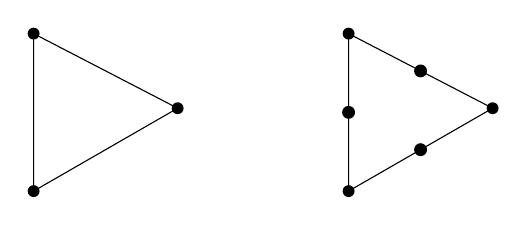
\begin{tikzpicture}[scale=1.0,dot/.style={draw,circle,fill=black,inner sep=1.5pt,pos=0.5}]
\newcommand{\ldot}{node[circle,fill=black,inner sep=0.5pt] (0.0pt) {.}}
\pgfmathsetmacro{\xo}{0.0}
\pgfmathsetmacro{\yo}{0.0}
  \draw[black] (0.000000+\xo,-2.000000+\yo) \ldot -- (1.828947+\xo,-0.947368+\yo) \ldot -- (0.000000+\xo,0.000000+\yo) \ldot -- (0.000000+\xo,-2.000000+\yo) ;
\pgfmathsetmacro{\xo}{4.0}
  \draw[black] (0.000000+\xo,-2.000000+\yo) \ldot -- node[dot](){}  (1.828947+\xo,-0.947368+\yo) \ldot -- node[dot](){} (0.000000+\xo,0.000000+\yo) \ldot -- node[dot](){} (0.000000+\xo,-2.000000+\yo) ;
\end{tikzpicture}
\caption{$P_1$ and $P_2$ elements.}
\label{fig:fedofs}
\end{figure}

A continuous function on $\Omega$ which is piecewise-linear on each triangle, i.e.~in $P_1$ on each triangle, is determined by its values at the $N_1$ nodes.  The space of such functions is a subspace $Q^h \subset Q$ of the pressure function space $Q$ used in the weak form \eqref{weak}; we say $Q^h$ is a $P_1$ space.

A continuous function on $\Omega$ which is piecewise-quadratic on each triangle, i.e.~in $P_2$ (Figure \ref{fig:fedofs}), is determined by its values at the nodes plus the edge midpoints \cite{Elmanetal2014}.  Let $N_2$ denote the number of all such nodes at which the solution is sought.  (The meshes used in numerical examples have Dirichlet boundaries, and these nodes are not included in $N_2$.)  A small example of this kind of mesh is shown in Figure \ref{fig:fedims}.

\begin{figure}[ht]
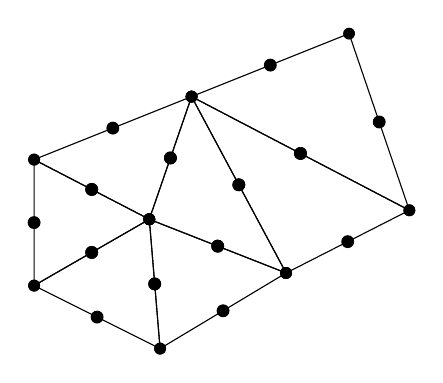
\begin{tikzpicture}[scale=0.8,dot/.style={draw,circle,fill=black,inner sep=1.5pt,pos=0.5}]
\pgfmathsetmacro{\xo}{0.0}
\pgfmathsetmacro{\yo}{0.0}
\newcommand{\ldot}{node[circle,fill=black,inner sep=0.5pt] (0.0pt) {.}}
  \draw[black] (0.000000+\xo,-2.000000+\yo) \ldot -- node[dot](){}  (1.828947+\xo,-0.947368+\yo) \ldot -- node[dot](){} (0.000000+\xo,0.000000+\yo) \ldot -- node[dot](){} (0.000000+\xo,-2.000000+\yo) ;
  \draw[black] (2.000000+\xo,-3.000000+\yo) \ldot -- node[dot](){} (1.828947+\xo,-0.947368+\yo) \ldot -- node[dot](){} (0.000000+\xo,-2.000000+\yo) \ldot -- node[dot](){} (2.000000+\xo,-3.000000+\yo) ;
  \draw[black] (0.000000+\xo,0.000000+\yo) \ldot -- node[dot](){} (1.828947+\xo,-0.947368+\yo) \ldot -- node[dot](){} (2.500000+\xo,1.000000+\yo) \ldot -- node[dot](){} (0.000000+\xo,0.000000+\yo) ;
  \draw[black] (1.828947+\xo,-0.947368+\yo) \ldot -- node[dot](){} (2.000000+\xo,-3.000000+\yo) \ldot -- node[dot](){} (4.000000+\xo,-1.799890+\yo) \ldot -- node[dot](){} (1.828947+\xo,-0.947368+\yo) ;
  \draw[black] (4.000000+\xo,-1.799890+\yo) \ldot -- node[dot](){} (5.957182+\xo,-0.804788+\yo) \ldot -- node[dot](){} (2.500000+\xo,1.000000+\yo) \ldot -- node[dot](){} (4.000000+\xo,-1.799890+\yo) ;
  \draw[black] (2.500000+\xo,1.000000+\yo) \ldot -- node[dot](){} (1.828947+\xo,-0.947368+\yo) \ldot -- node[dot](){} (4.000000+\xo,-1.799890+\yo) \ldot -- node[dot](){} (2.500000+\xo,1.000000+\yo) ;
  \draw[black] (2.500000+\xo,1.000000+\yo) \ldot -- node[dot](){} (5.957182+\xo,-0.804788+\yo) \ldot -- node[dot](){} (5.000000+\xo,2.000000+\yo) \ldot -- node[dot](){} (2.500000+\xo,1.000000+\yo) ;
\end{tikzpicture}

\caption{A mesh with $K=7$ elements, $N_1=8$ nodes, and $N_2=21$ edges.}
\label{fig:fedims}
\end{figure}

We define $V_0^h$ to be the space of \emph{pairs} of scalar piecewise-quadratic functions on $\Omega$, additionally requiring them to be zero on the base and inflow boundaries, i.e.~where \eqref{basebc} and \eqref{inflowbc} apply.  Thus functions from $V_0^h$ are 2D vector fields whose components are piecewise-quadratic scalar functions, i.e.~$P_2$ functions.  We define $V_D^h$ to be the nearly the same space except satisfying \eqref{inflowbc} on the inflow boundary.  Thus we have two $P_2$ velocity subspaces used in the weak form \eqref{weak}: $V_0^h \subset V_0$, $V_D^h \subset V_D$.

``Hat'' functions $\psi_j(x,z)$ form a convenient pressure test function basis (of $Q^h$).  Such functions are linear on each triangle, continuous on $\Omega$, equal to one at the one node $(x_j,z_j)$, and otherwise zero at the nodes, so that $\psi_j(x_i,z_i) = \delta_{ij}$.  (Figure 1.6 in \cite{Elmanetal2014} shows such a hat function.)  The set $\{\psi_j\}$ is a set of $N_1$ linearly-independent functions in $Q^h$.  Similarly, for every $P_2$ node which is not in the base or inflow boundary, whether a triangle vertex or edge midpoint, one defines a pair of basis functions for the velocity test space $V_0^h$.  These are pairs of piecewise-quadratic hat functions, $(\phi_j(x,z),0)$ or $(0,\phi_j(x,z))$; Figure 1.7 in \cite{Elmanetal2014} suggests how such $P_2$ hat functions would look.  These hat functions form a set of $2N_2$ linearly-independent functions in $V_0^h$.

Using $P_2$-$P_1$ elements the dimension of the velocity space is always higher than the pressure space, and often much higher.  For example, for the $N_1=356$ vertex mesh shown in Figure \ref{fig:glacier}, the velocity dimension $2N_2=2646$ is seven times greater than $N_1$.  Such a dimension imbalance turns out to be desirable!  As explained in the FE literature under the obscure name ``inf-sup condition'' \cite{Braess2007,Bueler2021,Elmanetal2014}, Stokes equations mixed methods are only stable if the velocity space is sufficiently-large relative to the pressure space.

The FE method itself, a finite-dimensional approximation of the weak form \eqref{weak}, can now be stated.  It seeks $\bu^h \in V_D^h$ and $p^h \in Q^h$ so that
\begin{equation}
F(\bu^h,p^h;\bv^h,q^h) = 0 \qquad \text{ for all } \bv^h\in V_0^h \text{ and } q^h\in Q^h  \label{feweak}
\end{equation}
Note that we have merely added ``$h$'' superscripts to all continuum quantities!  The nonlinear functional $F$ is unchanged, and it is computed concretely, though also approximately, by quadrature \cite{Bueler2021,Elmanetal2014}.  The FEM solution to \eqref{feweak} can be shown to be well-posed by the same theory that applies to the continuum problem \cite[Theorem 4.3]{JouvetRappaz2011}.  By linearity of $F$ in the $\bv,q$ positions, it suffices to consider only a basis of test functions from $V_0^h$ and $Q^h$.  A system of nonlinear, algebraic equations, the (sparse) discrete Glen-Stokes problem, is thus formed by requiring \eqref{feweak} to hold for all basis functions identified above.  These equations are assembled element-by-element in the sense that for each triangle $\triangle_k$ the contribution from that triangle is added to the correct equation \cite[Chapter 10]{Bueler2021}.

Nonlinear system \eqref{feweak} is solved by Newton's method \cite{Bueler2021,Kelley2003}.  At each Newton step we solve a sparse and indefinite linear system.  These systems have a well-known block structure (Figure \ref{fig:lowspy}), so we apply a Schur complement preconditioner in the GMRES Krylov iteration \cite{Elmanetal2014,GolubVanLoan2013}.  This buzzword salad is an indication of the complexity of solver technology, and we abandon further explanation here, but see \cite[Chapter 14]{Bueler2021}.

\begin{figure}[h]
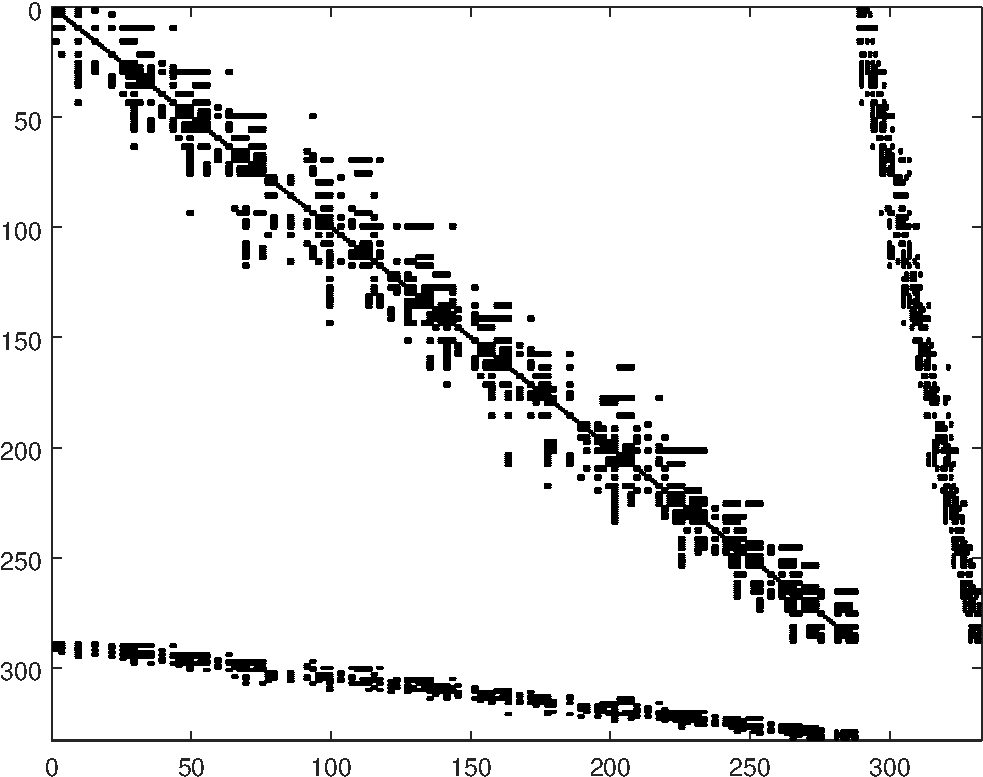
\includegraphics[width=0.45\textwidth]{lowspy}
%./domain.py -hmesh 300.0 -refine_corner 2 -o low.geo
%gmsh -2 low.geo
%./flow.py -mesh low.msh -s_mat_type aij -s_ksp_view_mat :low.m:ascii_matlab
% then spy() in Matlab
\caption{Sparsity pattern of the Newton step linear system, when solving the Stokes equations on a coarse mesh ($K=52,N_1=40,N_2=91$).}
\label{fig:lowspy}
\end{figure}

Our Python codes define the nonlinear residual function $F$ in \eqref{defineF} using the Firedrake/FEniCs domain-specific language for describing such weak forms \cite{Alnaesetal2014}.  Then we call the Firedrake method \texttt{solve()} on \eqref{feweak} \cite{Rathgeberetal2016}.  A practical view of our codes, including the sequence in which they are used in practice, and how they are divided into modules, is in the final section of these notes.


\section{Surface kinematical equation} \label{sec:kinematical}

A glacier will change shape as it flows, and as its surface simultaneously interacts with the climate (precipitation and melting).  We also want a model which includes this action!  So now suppose that the domain on which the Stokes equations apply is time-dependent:
\begin{equation}
\Omega^t = \left\{(x,z)\,\big|\, b(x) < z < s(x,t)\right\}  \label{Omegat}
\end{equation}
Here $z=b(x)$ is the base elevation and $z=s(x,t)$ is the ice surface elevation.

The time-dependent surface $z=s(x,t)$ evolves according to the surface kinematical equation, (41) in the notes, using ice velocity $\bu=\left<u(x,z,t),w(x,z,t)\right>$:
\begin{equation}
s_t = a(x,t) - u(x,s,t) s_x + w(x,s,t) \label{surfacekinematical}
\end{equation}
Here $a(x,t)$ is the climatic mass balance in units of ice-equivalent $\text{m}\,\text{s}^{-1}$.  Informally, \eqref{surfacekinematical} determines the change in surface elevation $\Delta s \approx s_t\,\Delta t$ from the climatically added/removed ice $a\,\Delta t$, \emph{plus} the component of the ice motion in the outward (upward) normal direction $\bn = \left<-s_x,1\right>$.  Thus $\Delta s \approx \left(a + \bn\cdot \bu|_{z=s}\right) \Delta t$.

Equation \eqref{surfacekinematical} applies on the time-dependent ice surface $\Gamma^t = \left\{(x,z) \,\big|\, z = s(x,t)\right\}$.  The surface $\Gamma^t$ is also the zero level surface of the function
    $$\Psi(x,z,t) = z - s(x,t)$$
\cite[pp.~65--66]{GreveBlatter2009}; we must regard $\Psi$ as being defined on the closure of $\Omega^t$, including the surface $\Gamma^t$.  Since the spatial gradient $\grad \Psi = \left<-s_x,1\right> = \bn$ is the same outward normal along $\Gamma^t$, we have
\begin{equation}
s_t = a + \bu|_{\Gamma^t} \cdot (\grad \Phi)|_{\Gamma^t}  \label{surfacekinematicalwithPhi}
\end{equation}
In Firedrake the advantage of using \eqref{surfacekinematicalwithPhi}, over \eqref{surfacekinematical}, is that it is easier to compute the gradient of the 2D scalar field $\Psi(x,z,t_n)$, and evaluate it along the boundary, than it is to differentiate the surface elevation function $s(x,t_n)$.

In our examples below, because we are studying ice fluid dynamics in isolation, we set $a=0$.  Scientific questions generally require nontrivial models for $a$.  Given such a model, implementation of nonzero values for $a(x,t)$ is straightforward if applied in an explicit (time-split) manner, which is what we do here.

Regarding the base, in our simplified model the elevation $b(x)$ is time-independent, and the base does not slide, nor does it melt/refreeze liquid water, and thus the base kinematical equation, (42) in the notes, reduces to ``$0=0$.''  Modifying our scheme to apply a nontrivial basal mass balance would not be difficult in our explicit time-stepping paradigm.

We can now describe our explicit time-stepping strategy for moving the surface of a glacier.  Namely, we take a time step of the surface kinematical equation \eqref{surfacekinematicalwithPhi} by smoothly displacing the mesh in the vertical direction only.  The mesh geometry is given by scalar coordinate fields $(x,z)$, defined on the nodes of the mesh.  At time $t_n$ the ice surface elevation $s^n(x) \approx s(x,t_n)$ equals the value of the coordinate field $z$ on the top boundary of the time $t_n$ mesh $\Omega^n$.  We determine the boundary value of a Laplace equation problem, for the vertical displacement $r^n$ of every node in the mesh, from \eqref{surfacekinematicalwithPhi}.

Given the current ($t_n$) geometry of the ice and a time step $\Delta t_n > 0$, apply this sequence:

\medskip
\renewcommand{\labelenumi}{\emph{\arabic{enumi}.}}
\begin{enumerate}
\item Solve the weak-form Stokes equation \eqref{weak} on the current mesh $\Omega^n$ to compute current velocity and pressure values $(\bu^n,p^n)$.
\item From $\Omega^n$ also generate the piecewise-linear surface elevation function $s^n(x)$.  Then evaluate $\Phi^n(x,z) = z - s^n(x)$ on $\Omega^n$ and compute:
\begin{equation}
\Delta s^n(x,z) =  \left(a(x,t_n) + \grad \Phi^n(x,z)\cdot \bu^n(x,z)\right)\Delta t_n \label{deltahfield}
\end{equation}
Note $\Delta s^n$ is defined on all of $\Omega^n$, not just the glacier surface.
\item Solve a Laplace equation problem for the vertical displacement field $r^n$:
\begin{align}
- \grad^2 r^n &= 0 & &\text{on } \Omega^n \label{vdisplacementpoisson} \\
          r^n &= \Delta s^n & &\text{(Dirichlet) on the top boundary } \Gamma^n \notag \\
          r^n &= 0 & &\text{(Dirichlet) on inflow and base of } \partial \Omega^n \notag \\
\grad r^n\cdot \bn &= 0 & &\text{(Neumann) on outflow of } \partial \Omega^n \notag
\end{align}
This linear problem is solved in weak form: $\int_{\Omega^n} \grad r^n\cdot \grad q = 0$ for all test functions $q$ with zero values on the Dirichlet part of the boundary $\partial \Omega^n$.
\item Update the mesh coordinates using vertical-only displacement by $r^n$:
\begin{equation}
  x^{n+1} = x^n, \quad z^{n+1} = z^n + r^n \label{updatemesh}
\end{equation}
\end{enumerate}

\medskip
At the end of this sequence the new top boundary $\Gamma^{n+1}$ is the updated surface $z=s^{n+1}(x)$.  By \eqref{deltahfield} the sequence has done an explicit step of \eqref{surfacekinematical}:
    $$s^{n+1}(x) = s^n(x) + \Delta t_n\,\left(a(x,t_n) - u(x,s^n,t_n) s_x^n + w(x,s^n,t_n)\right)$$

The significance of Dirichlet problem \eqref{vdisplacementpoisson} is that the entire mesh is \emph{smoothly} displaced, in the vertical direction only by \eqref{updatemesh}, because solutions of the Laplace equation are smooth.  Note $r^n$ minimizes $\int |\grad r^n|^2$ over functions with the given boundary values.  This way of displacing the mesh avoids shearing the mesh above sharp discontinuities in base topography, for example.

Our scheme uses fixed time step $\Delta t > 0$ and is explicit.  At best it can be conditionally stable, and in practice that \emph{is} what is observed, but no quantiative time step restriction is known; an \emph{a priori} method for setting the time step is not known.  For an SIA solver a sufficient condition like ``$D\Delta t / \Delta x^2 < 1$'' applies, where $\Delta x$ is a representative mesh spacing and $D$ is some diffusivity parameter.  However, there is no literature which connects the $D$ from the SIA (see the notes) with Stokes time-stepping, or otherwise supplies a stability restriction for surface-evolving Stokes models.

Two methods of addressing this numerical modeling weakness have, I think, barely been started by the glacier modeling community:
\renewcommand{\labelenumi}{(\roman{enumi})}
\begin{enumerate}
\item Extensively test various configurations to develop an empirical time-step restriction, depending on size and aspect-ratio of elements in some complicated way.
\item Solve the Stokes and surface kinematical equations in implicit-step form, as a coupled system.
\end{enumerate}
I am working on the latter!

\section{Implementation in Python codes} \label{sec:implementation}

We implement the above numerical solution method in Python codes.  These codes use the Firedrake FE \cite{Rathgeberetal2016} and PETSc solver libraries \cite{Balayetal2018,Bueler2021}.  Here is a simple example solving a time-independent Stokes problem:

\medskip
\begin{Verbatim}
$ ./domain.py -o glacier.geo                   # create domain outline
$ gmsh -2 glacier.geo                          # mesh domain
$ source ~/firedrake/bin/activate              # start Firedrake
(firedrake) $ ./flow.py -mesh glacier.msh      # solve Stokes problem
(firedrake) $ paraview glacier.pvd             # visualize results
\end{Verbatim}
%$

\medskip
\noindent In a time-stepping run one supplies the time step in days (\texttt{-deltat}) and the number of steps (\texttt{-m}).  For example, the following run generates the result shown in Figure \ref{fig:glacier}:

\medskip
\begin{Verbatim}
(firedrake) $ ./flow.py -mesh glacier.msh -deltat 20.0 -m 100
\end{Verbatim}
%$

\medskip
\noindent The \verb|README.md| file documents usage more thoroughly.

\medskip
As shown in Figure \ref{fig:blockdiagram} there are a total of five Python codes:
\begin{itemize}
\item \texttt{domain.py}: \quad  This writes an outline of the initial domain $\Omega^0$ into an ASCII file (\texttt{.geo} extension) using the Gmsh \cite{GeuzaineRemacle2009} geometry description language.  Note Gmsh can be used to examine and mesh this domain interactively or at the command-line, as above.  Portions of the boundary are marked with integer tags; see the Python dictionary \texttt{bdryids}.  This module also exports a function \texttt{getdomaindims()} which dynamically-extracts dimensions from a changing mesh.

\item \texttt{flow.py}: \quad  This driver reads user options, reads the mesh from a Gmsh \texttt{.msh} file, uses a \texttt{MomentumModel} object to solve the Stokes problem, optionally calls \texttt{meshmotion.py} to do the above time-stepping strategy, and writes the solution into a Paraview-readable \texttt{.pvd} file.

\item \texttt{meshmotion.py}: \quad  This module assembles and solves linear Dirichlet problem \eqref{vdisplacementpoisson} for vertical mesh displacement using Firedrake's \texttt{solve()}, and it updates the mesh coordinates as described.  This solver has option prefix \texttt{vd\_}.

\item \texttt{momentummodel.py}: \quad  Implements \texttt{class MomentumModel}.  Most actual ice physics is isolated here, including physical constants and the Stokes problem weak form \eqref{defineF}.  The \texttt{solve()} method of this class assembles and solves the nonlinear Glen-Stokes problem \eqref{weak} using Firedrake's \texttt{solve()} command.  This solver has option prefix \texttt{s\_}.

\item \texttt{surfaceutils.py}: \quad  Provides functions which extract boundary values of solution fields and mesh coordinates.  Note that the surface values of the solution can be visualized in a separate image file (e.g.~\texttt{.png}) using option \texttt{-osurface}.
\end{itemize}

\begin{figure}[h]
\bigskip
\tikzstyle{tool} = [draw, minimum size=2em]
\tikzstyle{module} = [draw, dashed, minimum size=2em]
\tikzstyle{other} = [draw, minimum size=2em, rounded corners=0.2cm]
\begin{tikzpicture}[node distance=3.8cm,>=latex]
    \node [tool]   (domain) {\texttt{domain.py}};
    \node [other]  (gmsh)[right of= domain] {Gmsh};
    \node [tool]   (flow)[right of=gmsh] {\texttt{flow.py}};
    \node [other]  (paraview)[right of=flow] {Paraview};
    \node [module] (momentummodel)[above left of=flow, xshift=-2.1cm] {\begin{minipage}{4.0cm} \texttt{momentummodel.py} \footnotesize (\texttt{class MomentumModule}) \end{minipage}};
    \node [module] (meshmotion)[above right of=flow, xshift=-3cm] {\texttt{meshmotion.py}};
    \node [module] (surfaceutils)[right of=meshmotion, xshift=0.3cm] {\texttt{surfaceutils.py}};
    \path[->] (domain) edge node[below] {\texttt{.geo}} (gmsh) ;
    \path[->] (gmsh) edge node[below] {\texttt{.msh}} (flow) ;
    \path[->] (flow) edge node[below] {\texttt{.pvd}} (paraview) ;
    \path[->] (domain) edge[dashed, bend left] node {} (flow) ;
    \path[->] (momentummodel) edge[dashed] node {} ([xshift=-0.2cm]flow.north) ;
    \path[->] (meshmotion) edge[dashed] node {} (flow) ;
    \path[->] (surfaceutils) edge[dashed] node {} (flow) ;
    \path[->] (surfaceutils) edge[dashed, bend right] node {} (meshmotion) ;
\end{tikzpicture}

\medskip
\caption{Users interact with tools (solid outlines) in the given order.}
\label{fig:blockdiagram}
\end{figure}


\small

\bigskip
\bibliography{stokes}
\bibliographystyle{siam}

\end{document}
